\section{Agda Mechanization}\label{sec:mechanization}
Thus far, we have presented a system for pattern matching with typed holes, and we have discussed the reasoning and motivation for all of its aspects. Hopefully, the reader should find our system fairly intuitive, and should be reasonably convinced of its correctness. Indeed, we have provided various metatheoretical and semantic theorems which indicate that all of our judgements behave as expected, and that they enforce the constraints we desire.

However, even with such theorems stated and proved on-paper, we must consider that humans have quite a propensity for error. (After all, much of our work here focuses on analyses which seek to prevent common human errors!) Indeed, pattern matching with holes in both expressions and patterns can be very intricate, requiring reasoning about a three-valued logic of must, must not, and indeterminate judgments. Likewise, the proofs of our theorems involve large amounts of casework, considering many combinations of expressions, patterns, and constraints. Anecdotally, our initial work required nearly 150 pages of tediously typed out proofs. Thus, while on-paper proofs \emph{supposedly} show that our system is correct, it is highly unlikely that such voluminous work is entirely error-free.

To address this, and to provide a stronger guarantee of our system's correctness, we then must utilize something much more reliable than human intuition. Namely, we turn to the Agda proof-assistant \cite{norell:thesis}, providing a computer-checked mechanization of nearly all theorems stated here. Our mechanization is available for viewing at \href{https://github.com/hazelgrove/patterns-agda}{https://github.com/hazelgrove/patterns-agda}, and it is well-commented with documentation explaining the contents of each file. The only results we do not mechanize are those related to the $\cincon{\Xi}$ procedure discussed in \autoref{sec:decidability}. As previously mentioned, such proofs involve algorithms which use finite sets sets in a non-structurally recursive way, making them cumbersome to implement in Agda.

Throughout the rest of this section, we present an in depth discussion of our mechanization. In \autoref{sec:dependent-types}, we review the general background for dependently type theorem provers. Next, in \autoref{sec:mech-details}, we discuss how we encode our judgements, giving particular attentions to choices regarding binders, contexts, and other aspects that are often glossed over on paper. Finally, in \autoref{sec:errors}, we reflect on the benefit of our mechanization, enumerating the various subtle errors it revealed. 

\subsection{Theorem Proving with Dependent Types}\label{sec:dependent-types}
To begin, we review the required background on the Agda proof-assistant, discussing how its type system enables users to mechanically verify mathematical propositions. All of the material here is standard and should be familiar to the academic programming language researcher.

Briefly, Agda and other dependently-typed proof assistants function based on the following key observation: a type $T$ may be regarded as representing a proposition "$T$ is inhabited", and constructing a term $\ctyp{t}{T}$ correspondingly provides a proof of this proposition. If  our type system is sufficiently rich, we also have the converse: for any proposition $P$, we may construct a type $T_P$ such that "$T_P$ is inhabited" is logically equivalent to $P$, and the terms of $T_P$ are exactly the proofs of $P$. With such a type system, there is a one-to-one correspondence between propositions and types and between proofs and terms, commonly known as the \emph{Curry-Howard Correspondence} \cite{howard1980formulae}. 

Considering Agda in particular, it is a typed functional programming language based on a variant of Martin-L\"of type theory \cite{DBLP:books/daglib/0000395} known as the Unified Theory of Dependent Types \cite{DBLP:books/daglib/0078470, norell:thesis}. With dependent types, the division between types and values becomes blurry - types may be parameterized by arbitrary values, and types may be given as arguments and results of functions. Such a formulation is quite powerful, allowing Agda's type system to correspond with a variant of intuitionistic logic. 

Let us show a small taste of the details of this correspondence. For a simple example, take binary product types $A \times B$. As terms of $A \times B$ are of the form $\hpair{a}{b}$ where $\ctyp{a}{A}$ and $\ctyp{b}{B}$, the terms of $A \times B$ consist exactly of a proof of $A$ and a proof of $B$. Thus, $A \times B$ corresponds to the logical "and" of propositions $A \times B$. Indeed, \autoref{fig:product-and} shows that the type checking rules for $A \times B$ syntactically mirror the intuitionistic natural deduction rules for $A \land B$.

% !TeX root = thesis.tex
\begin{figure}[ht]

\begin{mathpar}
\Infer{\AndIntro}{ 
	\Gamma \vdash A \\ \Gamma \vdash B 
}{
	\Gamma \vdash A \land B
}

\Infer{\AndElimL}{
	\Gamma \vdash A \land B
}{
	\Gamma \vdash A
}

\Infer{\AndElimR}{
	\Gamma \vdash A \land B
}{
	\Gamma \vdash B
}

\Infer{\TAPair}{
	\Gamma \vdash a : A\\ \Gamma \vdash b : B
}{
	\Gamma \vdash (a, b) : A \times B
}

\Infer{\TAFst}{
	\Gamma \vdash p : A \times B
}{
	\Gamma \vdash \hfst{p} : A
}

\Infer{\TAFst}{
	\Gamma \vdash p : A \times B
}{
	\Gamma \vdash \hsnd{p} : B
}
\end{mathpar}
	
\caption{Correspondence between $A \times B$ and $A \land B$}
\label{fig:product-and}
\end{figure}


Analogously, binary sums $A + B$ correspond to the logical "or" of propositions $A \lor B$. For a more interesting case, consider propositions of the form $\forall x. B$, stating that for any $x$, the proposition $B$ holds, where $B$ may depend on $x$. In our correspondence, we can consider $B$ to be a type parameterized by a value $x$, say $x : A$ for some other type $A$. That is, $B$ is a \emph{dependent type}. To prove $\forall x..~ B$, we then must be able to produce a proof $f(a) : [a / x]B$ for any $a : A$. That is, we should have a function $f$ which takes inputs $a : A$ and produces outputs $f(a) : [a / x]B$. We refer to $f$ as a \emph{dependent function}, noting that its return type may depend on the particular value of its input. Formally, we write $f : \Pi_{x : A} B$. \autoref{fig:function-forall} shows a syntactic correspondence between type checking rules for dependent functions and natural deduction rules for universal quantification. 

% !TeX root = thesis.tex
\begin{figure}[ht]
	
	\begin{mathpar}
		\Infer{\UniversalIntro}{ 
			\Gamma \vdash B \\ \text{($x$ not free in $\Gamma$)}
		}{
			\Gamma \vdash \forall x. B
		}
		
		\Infer{\UniversalElim}{
			\Gamma \vdash \forall x. B
		}{
			\Gamma \vdash [a / x]B
		}
		
		\Infer{\TALam}{
			\Gamma , x : A \vdash b : B
		}{
			\Gamma \vdash \lambda x : A. b : \Pi_{x : A} B
		}
		
		\Infer{\TAAp}{
			\Gamma \vdash f : \Pi_{x : A} B \\ \Gamma \vdash a : A
		}{
			\Gamma \vdash f(a) : [a / x] B
		}
	\end{mathpar}
	
	\caption{Correspondence between $\Pi_{x : A} B$ and $\forall x. B$}
	\label{fig:function-forall}
\end{figure}


With the general idea of this correspondence now clear, let us present another feature of Agda we use pervasively in our development: \emph{inductive type families}. Briefly, an inductive type $T$ is specified by a finite list of functions with return type $T$, called \emph{constructors}, and the terms of $T$ consist of any syntactic form built up freely by repeated application of these constructors. In particular, the constructors themselves may inductively take arguments from $T$.

For example, recall the Peano construction of the natural numbers, where a natural number is either $0$ or inductively the successor of another natural number $suc(n)$. In Agda, we can represent this as an inductive type \li{Nat} as defined in \autoref{fig:naturals}. Here, there are two constructors: \li{zero} which takes no arguments, and \li{suc} which inductively takes a single argument of type $Nat$. The terms of \li{Nat} are then of the form \li{zero},\; \li{suc zero},\; \li{suc (suc zero)}, and so forth. Formally, the constructors yield the introduction rules shown in \autoref{fig:naturals}, and while not enumerated, appropriate elimination rules are also added, allowing functions to be defined by handling the case of each different constructor.

% !TeX root = thesis.tex
\begin{figure}[h]
\begin{subfigure}{.45\textwidth}
	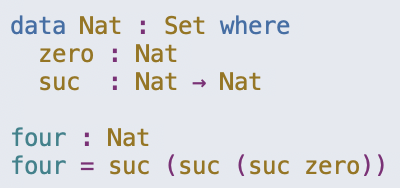
\includegraphics[scale=0.75,valign=t]{imgs/naturals.png}%
	\caption{Inductive Type Definition}
\end{subfigure}
\begin{subfigure}{.45\textwidth}
	\begin{mathpar}
		\Infer{\Zero}{
		}{
			\Gamma \vdash zero : Nat
		}\\
		\Infer{\Suc}{
			\Gamma \vdash n : Nat
		}{
			\Gamma \vdash suc~n : Nat
		}
	\end{mathpar}
	\caption{Introduction Rules}
\end{subfigure}
\caption{Natural numbers in Agda}
\label{fig:naturals}
\end{figure}

Inductive type families similarly define a family of types $T$, where $T$ may is parameterized by values or other types. With such types, we can easily encode almost any mathematical judgement, letting $T$ represent the judgement and the constructors of $T$ represent the defining inference rule. For example, we can define a type $x < y$ parameterized by values $x~y : Nat$, specifying that $x$ is less than $y$. For any such $x, y$, one can prove $x < y$ either by the fact that $0 < n$, or by inductively using the fact that $m < n$ to get that $suc~m < suc~n$. Correspondingly, \autoref{fig:naturals-ordering} defines an inductive type family $\_{<}\_ : Nat \to Nat \to Set$ with two constructors, also displaying the relevant inference rules. Here, the syntax $\_{<}\_$ is a \emph{mixfix operator} where each $\_$ denotes an argument position and $x < y$ desugars to $\_{<}\_~x~y$. Additionally, arguments written with curly braces in the form $\{x : Nat\}$ are implicit and inferred by the compiler.

% !TeX root = thesis.tex
\begin{figure}[ht]
	\begin{subfigure}{.45\textwidth}
		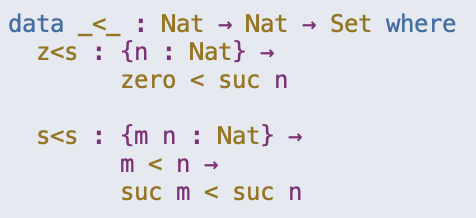
\includegraphics[scale=0.75,valign=t]{imgs/naturals-ordering.png}%
		\caption{Inductive Type Definition}
	\end{subfigure}
	\begin{subfigure}{.45\textwidth}
		\begin{mathpar}
			\Infer{\ZLessThanS}{
				\Gamma \vdash n : Nat
			}{
				\Gamma \vdash z{<}s : zero < suc~ n
			}\\
			\Infer{\SLessThanS}{
				\Gamma \vdash  m : Nat \\ \Gamma \vdash n : Nat \\ \Gamma \vdash p :  m < n
			}{
				\Gamma \vdash s{<}s~p : suc~m < suc~n
			}
		\end{mathpar}
		\caption{Introduction Rules}
	\end{subfigure}
	\caption{Ordering of natural numbers}
	\label{fig:naturals-ordering}
\end{figure}

\pagebreak

Considering our correspondence, we can then prove statements such as $\forall n \in \mathbb{N}, n < suc(n)$ by constructing a term of type $\Pi_{n : Nat}~n < suc~n$ as displayed in \autoref{fig:naturals-ordering-proof}. Note that Agda uses a more lightweight syntax for dependent function types $(n : Nat) \to  n < suc~n$.  The function is defined by pattern matching, handling the case of each constructor analogously to an induction on derivations. Exhaustiveness checking guarantees that all cases are handled.

% !TeX root = thesis.tex
\begin{figure}[ht]
	\centering
	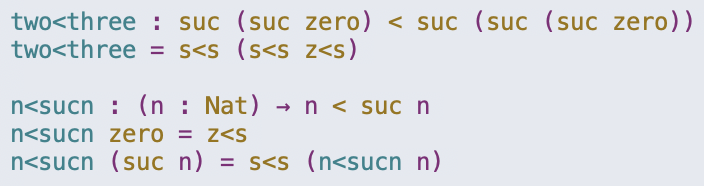
\includegraphics[scale=0.75,valign=t]{imgs/naturals-ordering-proof.png}%
	\caption{Example proofs using the ordering relation}
	\label{fig:naturals-ordering-proof}
\end{figure}

\subsection{Mechanization of Peanut}\label{sec:mech-details}
We are now ready to discuss the specifics of how we encode Peanut into Agda. Beginning with syntax, we can straightforwardly translate our grammar into an inductive data type. We utilize mixfix operators and Agda's unicode support in order to closely mirror the on-paper notation.

\todo{Show syntax definition}


\todo{Show constraint definition}

% Show syntax definition

% Show definition of simple judgement

% Discuss definition of contexts, function extensionality

% Discuss alpha equivalence, Barendregt's convention. Show binders disjoint definition,  example theorem assuming disjointness. Discuss subtlety related to substiuttions

\subsection{Issues Revealed by Mechanization}\label{sec:errors}
% Discuss  simple typos - IPrl and IRpp
% Discuss IPrl needing not a pair assumption
% Discuss xi possible judgemnet
% Discuss ITAp, val -> final, missing ITFst ITSnd

% Discuss 

% Discuss positivity issue reequiring us to separate analyses from type system

